\documentclass[UTF8,a4paper,10pt]{ctexart}
\usepackage[margin=2cm]{geometry}
\usepackage{fontspec,graphicx,caption}
\setmainfont{Times New Roman}
\setCJKmainfont[BoldFont=SimHei]{SimSun}
\pagestyle{empty}
\setlength{\parindent}{2em}
\setlength{\parskip}{3pt}
\captionsetup{font=small,skip=4pt}
\begin{document}
\fontsize{10.5}{15}\selectfont
为说明种植决策如何受农业条件约束、如何形成收益，以及三问分别改变了哪些参数和关系，本文将共享模型结构及其扩展概括于图1。

\begin{center}
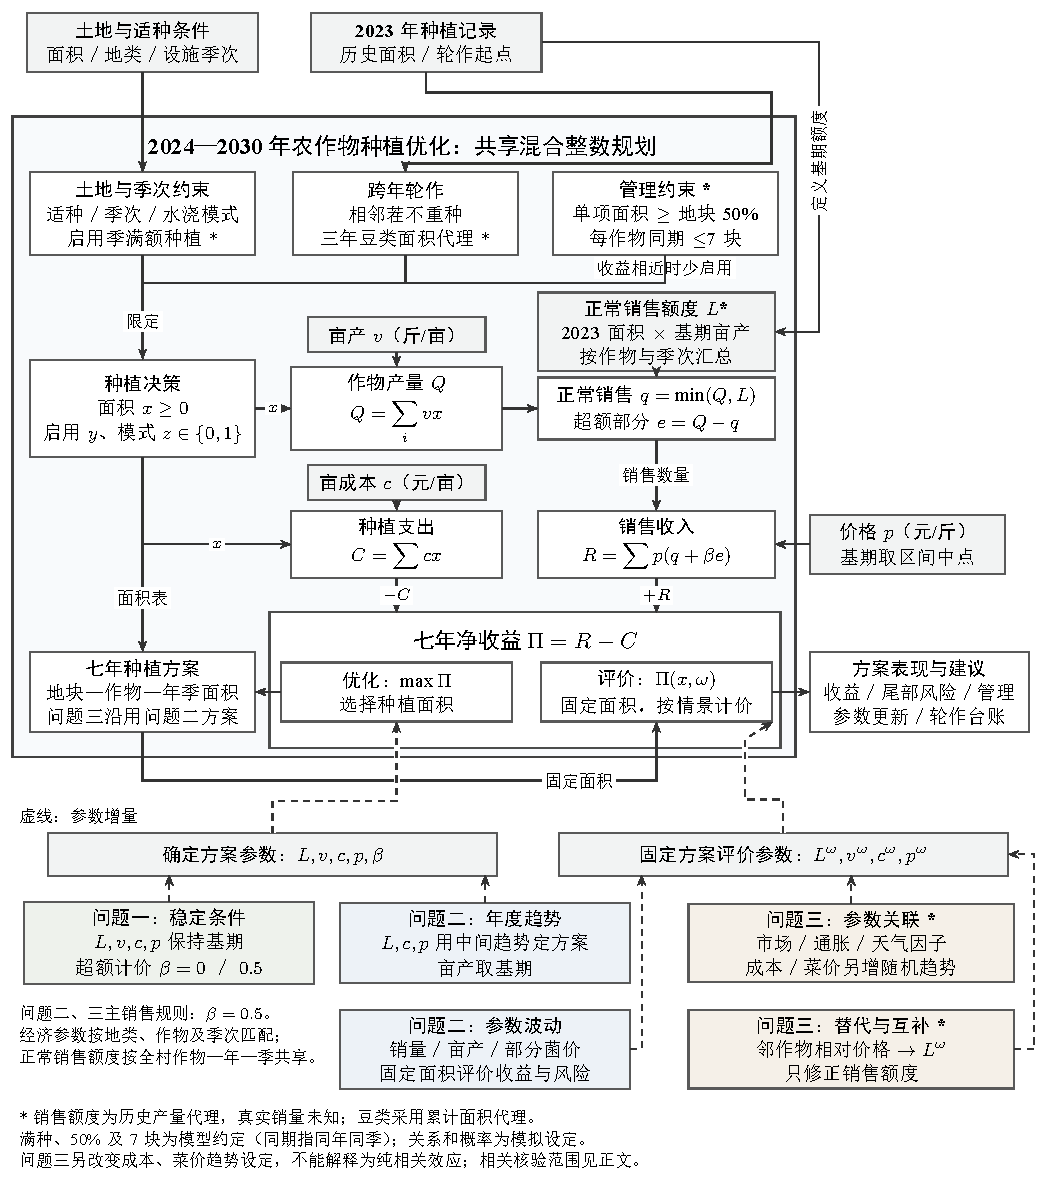
\includegraphics[width=17cm]{final_v2/model_framework.pdf}
\captionof{figure}{农作物种植优化的共享模型结构与三问增量}
\end{center}

图中的核心是共同的种植优化模型：面积、启用和水浇模式变量受土地、季次、轮作及管理约束限定；面积与亩产形成产量，产量和正常销售额度共同决定正常销售及超额部分，按相应价格规则形成收入，扣除种植支出后得到七年收益。问题一固定基期参数并比较两种超额计价规则；问题二以中间趋势参数确定种植方案，再用波动情景评价收益与尾部风险；问题三沿用问题二方案，将潜在因子相关和交叉价格需求响应作用于同一套产销计算。问题三还随机化了成本和蔬菜价格趋势，不能解释为纯相关效应。销量代理和合成关系均为条件分析设定。后文先说明参数来源与基本假设，再展开共享模型及各问扩展。
\end{document}
